%%%%%%%%%%%%%%%%%%%%%%%%%%%%%%%%%%%%%%%%%%%%%%%%%%%%%%%%%%%%%%%%%%%%%%%%%%%
%%                                                                       %%
%%     LaTeX + CTeX 《数学杂志》论文模板, 只针对 A4 纸的中文Paper.      %%
%%                                                                       %%
%%                                                                       %%
%%                                                          2006.3.1     %%
%%     版本历史:                                                         %%
%%        Ver0.01   2005.09.10                                           %%
%%        Ver1.01   2006.03.01                                           %%
%%               1. 更改编号出现错位                                     %%
%%               2. 增加作者信息                                         %%
%%               3. 调整首页标题、作者和摘要之间的间距                   %%
%%     You can mofify it and distribute it freely                        %%
%%                                                                       %%
%%%%%%%%%%%%%%%%%%%%%%%%%%%%%%%%%%%%%%%%%%%%%%%%%%%%%%%%%%%%%%%%%%%%%%%%%%%

%%%%%%%%%%%%%%%%%%%%%%%%%%%%%%%%%%%%%%%%%%%%%%%%%%%%%%%%%%%%%%%%
%            英文稿 文章模板:A4 纸, 小五字, 单列              %
%%%%%%%%%%%%%%%%%%%%%%%%%%%%%%%%%%%%%%%%%%%%%%%%%%%%%%%%%%%%%%%%
\documentclass[A4paper,11pt,onecolumn,twoside]{ctexart}
\usepackage{amsmath,amssymb,amsfonts,amsthm,fancyhdr}
\usepackage{epsfig,graphicx,picins,picinpar,subfigure}
\usepackage{pstricks}
\usepackage{fancyvrb}
\usepackage[numbers,sort&compress]{natbib}
\headsep=0.5truecm \footskip 0pt \topmargin 0pt \oddsidemargin 0pt
\evensidemargin 0pt \setlength{\textwidth}{14.8truecm}
\setlength{\textheight}{21.5truecm}
\renewcommand{\theequation}{\arabic{section}.\arabic{equation}}
\setcounter{page}{1}
 \pagestyle{fancy} \fancyhf{}
\renewcommand{\headrulewidth}{0.4pt}
%%%%%%%%%%%%%%%%%%%%%%%%%%%%%%%%%%%%%%%%%%%%%%%%%%%%%%%%%%%%%%%%
%        文章正文                                              %
%%%%%%%%%%%%%%%%%%%%%%%%%%%%%%%%%%%%%%%%%%%%%%%%%%%%%%%%%%%%%%%%

\begin{document}

\CTEXoptions[figurename={Figure}] \CTEXoptions[tablename={Table}]
\CTEXoptions[bibname={\normalsize References}]                % 加载自定义文件

%\apsnumber{2006/xxx}                       % 你的论文编号 --- 编辑部受理后产生

%%%%%%%%%%%%%%%%%%%%%%%%%%%%%%%%%%%%%%%%%%%%%%%%%%%%%%%%%%%%%%%%
%%-------------------- 作者提供的信息 ------------------------%%
%%%%%%%%%%%%%%%%%%%%%%%%%%%%%%%%%%%%%%%%%%%%%%%%%%%%%%%%%%%%%%%%
\newcommand{\authors}{}  % 仅用于页眉, 与\author{}中的一致 -- 用中文
%\newcommand{\mytitle}{论文题目}            % 仅用于页眉, 与\title{}中的一致 -- 用中文


%%%%%%%%%%%%%%%%%%%%%%%%%%%%%%%%%%%%%%%%%%%%%%%%%%%%%%%%%%%%%%%%
% 标题,作者, 通信地址定义
%%%%%%%%%%%%%%%%%%%%%%%%%%%%%%%%%%%%%%%%%%%%%%%%%%%%%%%%%%%%%%%%
%%\begin{CJK}{GBK}{song}
\title{\Large\textbf{ENGLISH TITLE}
\footnotetext[1]{\zihao{-5}\textbf{ Received date:}
XXXX-XX-XX\quad
                \quad \quad \textbf{ Accepted date:}XXXX-XX-XX}
\footnotetext[0]{\zihao{-5}\textbf{ Foundation item:} Supported by
                 National Natural Science Foundation of China(10671182).}
\footnotetext[0]{\zihao{-5}\textbf{ Biography:}
第一作者(出生时间--), 性别, 民族(汉族省写), 籍贯, 职称,
主要研究方向: xxxxxx. E-mail:xxxxx@xxxx.xxx.xx.}}





%%%%%%%%%%%%%%%%%%%%%%%%%%%%%%%%%%%%%%%%%%%%%%%%%%%%%%%%%%%%%%%%
% 作者姓名与单位 : 三种形式中选一种
% 后面中文摘要中的名字和单位同样处理
% ---------------------
% 第一种形式: 单一作者
% ---------------------
%\author{\textsc{Author1}\\[-1pt]
%(\textit{\zihao{-5} Author's Working Unit (Up to Department), Province Zip ~ Code}) \\[-2pt]}

% ---------------------
% 第二种形式: 同一单位 多个作者 -- 名字左右并列,
% ---------------------
\author{\zihao{5}{Author${^{1,2}}$,  Author2${^{2}}$}\\[-1pt]
(\textit{\zihao{-5} 1.Authors' Working Unit (Up to Department), Province Zip ~ Code, China}) \\[-2pt]
(\textit{\zihao{-5} 2.Authors' Working Unit (Up to Department), Province Zip ~ Code, China}) \\[-2pt]}

% ---------------------
% 第三种形式: 不同单位 多个作者 -- 名字与单位上下并列
% ---------------------
%\author{\textsc{Author1}\\[-1pt]
%(\textit{\zihao{-5} First Author's Working Unit (Up to Department), Province Zip ~ Code}) \\[-2pt]
%\textsc{Author2}\\[-1pt]
%(\textit{\zihao{-5} Second Author's Working Unit (Up to Department), Province Zip ~ Code}) \\[-2pt]}
%%%%%%%%%%%%%%%%%%%%%%%%%%%%%%%%%%%%%%%%%%%%%%%%%%%%%%%%%%%%%%%%

\date{}  % 这一行用来去掉默认的日期显示
\maketitle \vspace{-8mm}

%%%%%%%%%%%%%%%%%%%%%%%%%%%%%%%%%%%%%%%%%%%%%%%%%%%%%%%%%%%%%%%%
%  英文文摘要
%%%%%%%%%%%%%%%%%%%%%%%%%%%%%%%%%%%%%%%%%%%%%%%%%%%%%%%%%%%%%%%%
\begin{center}
\begin{minipage}[c]{14cm}
%\begin{center}\textbf{Abstract}\quad \end{center}
%\vspace{-1em}
\zihao{-5}
\mbox{}\hspace{2.3em}\textbf{Abstract: }
Here is the abstract... ... .\\
\mbox{}\hspace{2.3em}\textbf{Keywords:}\quad Keyword 1; Keyword 2; Keyword 3; Keyword 4.\\
\mbox{}\hspace{2.3em}\textbf{2010 MR  Subject Classification:}\quad XXXX ; XXXX\\
\mbox{}\hspace{2.3em}\textbf{Document code:\quad A \quad
\quad\quad\quad Article ID:\quad0255-7797(xxxx)0x-xxxx-xx}
\end{minipage}
\end{center}

%%%%%%%%%%%%%%%%%%%%%%%%%%%%%%%%%%%%%%%%%%%%%%%%%%%%%%%%%%%%%%%%
%  正文由此开始
%%%%%%%%%%%%%%%%%%%%%%%%%%%%%%%%%%%%%%%%%%%%%%%%%%%%%%%%%%%%%%%%
\zihao{5}
%%%%%%%%%%%%%%%%%%%%%%%%%%%%%%%%%%%%%%%%%%%%%%%%%%%%%%%%%%%%%%%%
%\vspace{1mm}


\vskip 2mm \noindent {\large {\bf 1 ~Introduction}} \vskip 3mm
\setcounter{section}{1}\setcounter{equation}{0}
%%%%%%%%%%%%%%%%%%%%%%%%%%%%%%%%%%%%%%%%%%%%%%%%%%%%%%%%%%%%%%%%

%%%%%%%%%%%%%%%%%%%%%%%%%%%%%%%%%%%%%%%%%%%%%%%%%%%%%%%%%%%%%%%%
\vskip 4mm \noindent {\large {\bf 2 ~A New Section}} \vskip 3mm
\setcounter{section}{2}\setcounter{equation}{0}
%%%%%%%%%%%%%%%%%%%%%%%%%%%%%%%%%%%%%%%%%%%%%%%%%%%%%%%%%%%%%%%%

Here are some examples of formulae, tables, figure insertions,
citations for your reference (see [1]).
\begin{equation} \label{eq:1}
\left\{ \begin{aligned}
         \pi &= 3.141\cdots \\
     \sqrt{2}&=1.414\cdots
         \end{aligned} \right.
\end{equation}

\begin{eqnarray}
         \pi &=& 3.1415926\cdots \nonumber \\
             &\approx & 3.14.
\end{eqnarray}



$$\begin{aligned}
         \pi &= 3.1415926\cdots \\
             &\approx  3.14.
\end{aligned}$$


$$\begin{aligned}
         \pi &= 3.1415926\cdots  \\
             &\approx  3.14.
\end{aligned}\eqno(3)$$




\begin{figure}[htbp]
\centering
\includegraphics[width=10cm,height=3cm]{figs/sin.eps}\\
\small{figure 1: A floating figure}
\end{figure}


\begin{figure}[htbp]
\begin{minipage}[t]{0.45\linewidth}
\centering
\includegraphics[width=6cm,height=3cm]{figs/sin.eps}\\
\small{figure 2: The first subfigure}
\end{minipage}%
\hfill
\begin{minipage}[t]{0.5\linewidth}
\centering
\includegraphics[width=5cm,height=3cm]{figs/fig.eps}\\
\small{figure 3: The second subfigure}
\end{minipage}
\end{figure}

{\bf Definition~ 2.1}~[2]~~~   This the definition... .



{\bf Lemma~ 2.2}~ (see [3])~~~  Here is the content of the lemma.




{\bf Theorem~ 2.3~~~}  Here is the content of the theorem.




{\bf Proof~~~}   Here comes the proof of the theorem.



{\bf Corollary~  2.4~~~}  Here is the content of the corollary.




Now comes some examples about citation:


{\bf Example~  1~~~}  See formula (2.1) on page 1.


\begin{center}
 {\small Table~1~~   $\gamma$~~~ Numerical Results}
 \vskip 2mm
\begin{tabular}{ccccc}
  \hline
  CPU Quantity & the number of iterations &   $\gamma^*$ & run time (second) \\
 \hline
   $10$ &  $3+57$ &         $ 2.2564$ & $1.22$\\
   $15$ &   $3+66$ &          $0.8235$ &  $1.35$\\
    $20$ &    $3+65$ &        $ 0.6421$ & $1.38$\\
  \hline
  \end{tabular}
%}
\end{center}


%%%%%%%%%%%%%%%%%%%%%%%%%%%%%%%%%%%%%%%%%%%%%%%%%%%%%%%%%%%%%%%%
\vskip 4mm \noindent {\large {\bf 3 ~ New Section}} \vskip 3mm
\setcounter{section}{3}\setcounter{equation}{0}

%%%%%%%%%%%%%%%%%%%%%%%%%%%%%%%%%%%%%%%%%%%%%%%%%%%%%%%%%%%%%%%%
{\bf Remark~~}  For further study on the typesetting based on
English-Chinese \LaTeX and some special techniques, we may refer
to [1--4].

\vspace{4mm}
%%%%%%%%%%%%%%%%%%%%%%%%%%%%%%%%%%%%%%%%%%%%%%%%%%%%%%%%%%%%%%%%
%  参考文献
%%%%%%%%%%%%%%%%%%%%%%%%%%%%%%%%%%%%%%%%%%%%%%%%%%%%%%%%%%%%%%%%
\zihao{-5}
\begin{thebibliography}{99}
%\setlength{\parskip}{0pt}  %段落之间的竖直距离
\addtolength{\itemsep}{-0.8 em} % 缩小参考文献间的垂直间距
  \bibitem{1}  Feller W.  An introduction to probability theory and its applications (3rd ed.)[M]. New York: Wiley, 1969.
  \bibitem{2}   Dawande M, Geismar H  N, Hall N G. Supply chain
scheduling: distribution systems [J]. Operations Research, 2007,
47(5): 511--517.
  \bibitem{3}  Xie Peng, Jiang Jun. Double chord-power integrals
  of a convex body and their applocations[A]. Eric L Grinberg.
  Integral geometry and convexity[C]. WHackensack, NJ: World Sci. Publ.,
   2006:  177--188.
  \bibitem{4}  王明亮. 关于中国学术期刊标准化数据库系统工程的进展[EB/OL].
  http//www.cajcd.edu.cn/pub/wml.txt/980810-2.html, 1998-08-16/1998-10-04.
  \end{thebibliography}

%%其中chinesebst是我自己生成的参考文献风格,比较符合中国人的习惯
%%参考文献
%% plain,unsrt,alpha,abbrev,chinesebst
%\bibliographystyle{chinesebst}
%\addtolength{\itemsep}{-0.5 em} % 缩小参考文献间的垂直间距
%%\bibliography{reference/reference,reference/chinese,reference/english}
%\bibliography{refs/aps_ref}


%%%%%%%%%%%%%%%%%%%%%%%%%%%%%%%%%%%%%%%%%%%%%%%%%%%%%%%%%%%%%%%%
%  英文摘要
%%%%%%%%%%%%%%%%%%%%%%%%%%%%%%%%%%%%%%%%%%%%%%%%%%%%%%%%%%%%%%%%
\vspace{4mm}\hspace{-8mm}
\parbox{\textwidth}{
\begin{center}
\Large{\textbf{论文题目 }}\\
\vspace{4mm}
\zihao{5}\textsc{第一作者$^{1,2}$~,~第二作者$^{2}$}\\[2pt]
({\zihao{-5}1.作者单位(到部门),~省~市~~ 邮政编码})\\[2pt]
({\zihao{-5}2.作者单位(到部门),~省~市~~ 邮政编码})\\[2pt]
\end{center}

\mbox{}\hspace{2em}{\CJKfamily{hei}~摘\,要:}\quad
本文研究了$\cdots\cdots$的问题. 利用$\cdots\cdots$的方法,
获得了$\cdots\cdots$结果,
推广了$\cdots\cdots$结果(即对结果的分析).}\\
\mbox{}\hspace{2em}{\CJKfamily{hei}关\,键\,词:}\quad 关键词1; 关键词2; 关键词3; 关键词4\\
\mbox{}\hspace{2em}{\CJKfamily{hei}MR(2010)主\,题\,分\,类\,号:}\quad
XXXX ;~XXXX
\mbox{}\hspace{2.4em}{\CJKfamily{hei}中\,图\,分\,类\,号:}\quad XX
;~XX


%%%%%%%%%%%%%%%%%%%%%%%%%%%%%%%%%%%%%%%%%%%%%%%%%%%%%%%%%%%%%%%%
%  文章结束
%%%%%%%%%%%%%%%%%%%%%%%%%%%%%%%%%%%%%%%%%%%%%%%%%%%%%%%%%%%%%%%%
\clearpage
%%\end{CJK*}
\end{document}
